\setlength{\columnsep}{5pt}
\begin{flushleft}
	\bigskip
	\bigskip
	\paragraph{What is a console and terminal?}
	\begin{itemize}
		\item A console is a device with a screen and keyboard combined inside it.
		\item Terminal is the software program inside the console.
			\begin{figure}[h!]
			\centering
			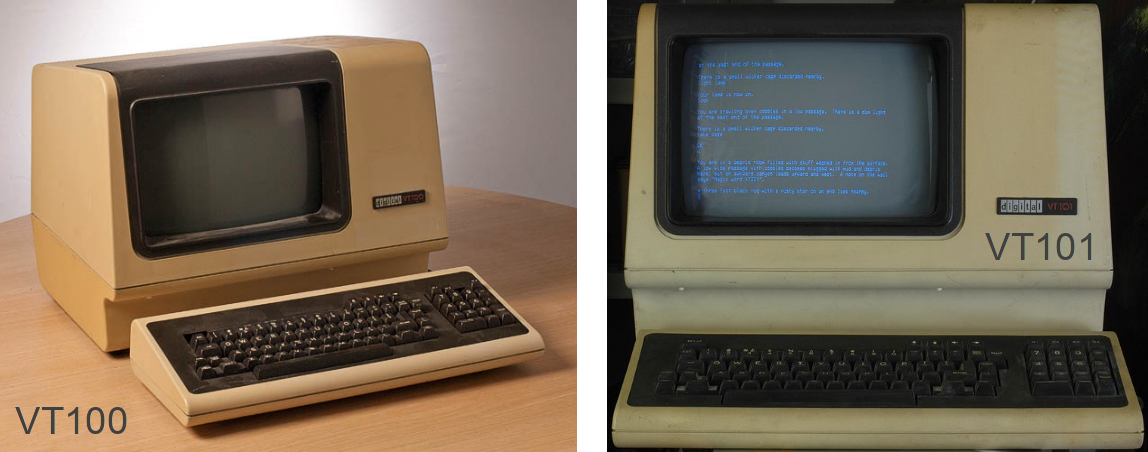
\includegraphics[width=5cm]{content/chapter1/images/console.png}
			\caption{VT terminals - The first console with terminal}%
			\label{fig:example}%
			\end{figure}		
	\end{itemize}
% figure side by side
%	\begin{figure}[h!]
%		\centering
%		\subfloat[\centering VT terminals]{{
%		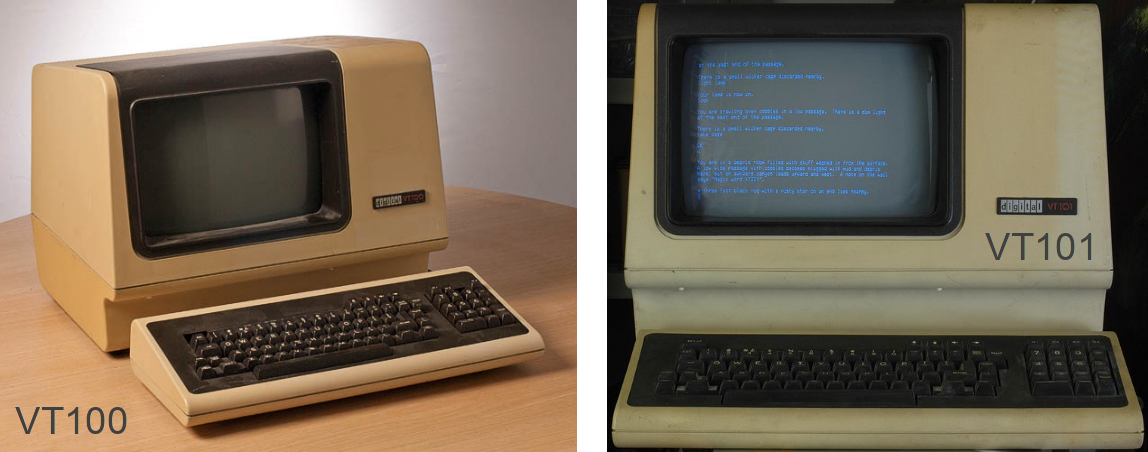
\includegraphics[width=10cm]{content/chapter1/images/console.png}}}%
%		\qquad
%		\subfloat[\centering RS-232 connector to connect console to terminal]{{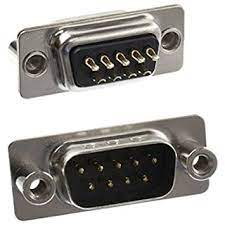
\includegraphics[width=5cm]{content/chapter1/images/connector.jpeg} }}%
%		\caption{2 VT terminal and connector}%
%		\label{fig:example}%
%	\end{figure}

	\paragraph{What is a command line?}
	\begin{itemize}
		\item It is a blank line and cursor on the screen, allowing the user to type commands to execute.
	
		\begin{figure}[h!]
			\centering
			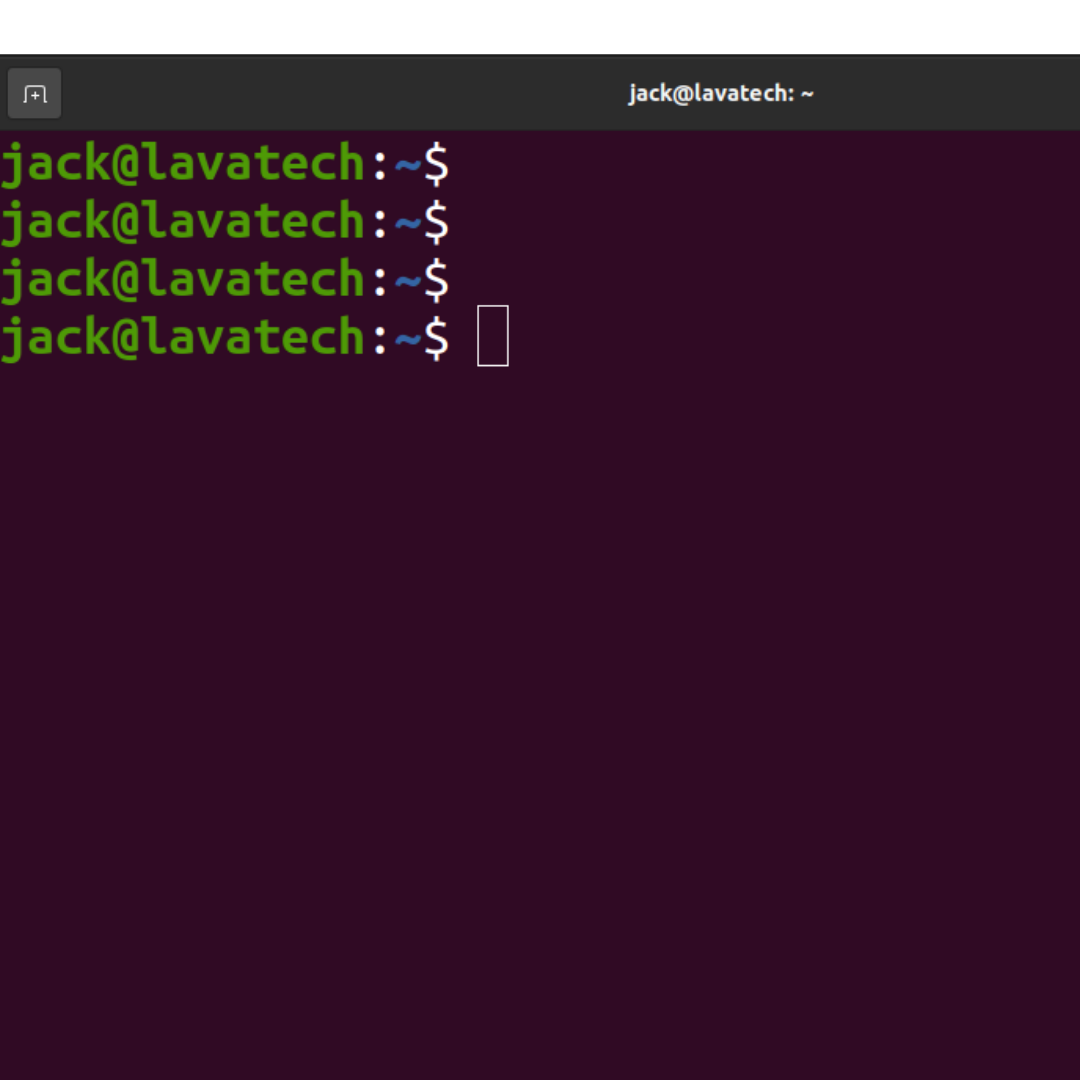
\includegraphics[scale=.18]{content/chapter1/images/commandline.png}
			\caption{Linux command line}
			\label{fig:commandline}
		\end{figure}	
	\end{itemize}
	\paragraph{What is a shell?}
	\begin{itemize}
		\item Shell is an interface to kernel.
		\item It executes Linux commands \& display it's result.
		\item Eg:
		\begin{itemize}
			\item Shell in Linux OS: bash, fish, zsh, ksh, sh, tsch
			\item Shell in Windows OS: PowerShell, pwsh
		\end{itemize}
	\end{itemize}		
\end{flushleft}

\newpage
